% TikZ: decision tree (binary classifier example)
\documentclass{article}
\usepackage{tikz}
\usetikzlibrary{shapes.geometric, positioning, arrows.meta}

\tikzset{
  internal/.style={rectangle, draw=blue!70, fill=blue!10, thick,
    rounded corners=3pt, minimum width=3cm, minimum height=0.85cm,
    text centered, font=\small},
  leaf/.style    ={ellipse, draw=green!60!black, fill=green!12, thick,
    minimum width=2.2cm, minimum height=0.85cm,
    text centered, font=\small},
  edge label/.style={font=\scriptsize, midway},
  arrow/.style={thick, -{Stealth[length=5pt]}},
}

\begin{document}
\begin{figure}[h]
\centering
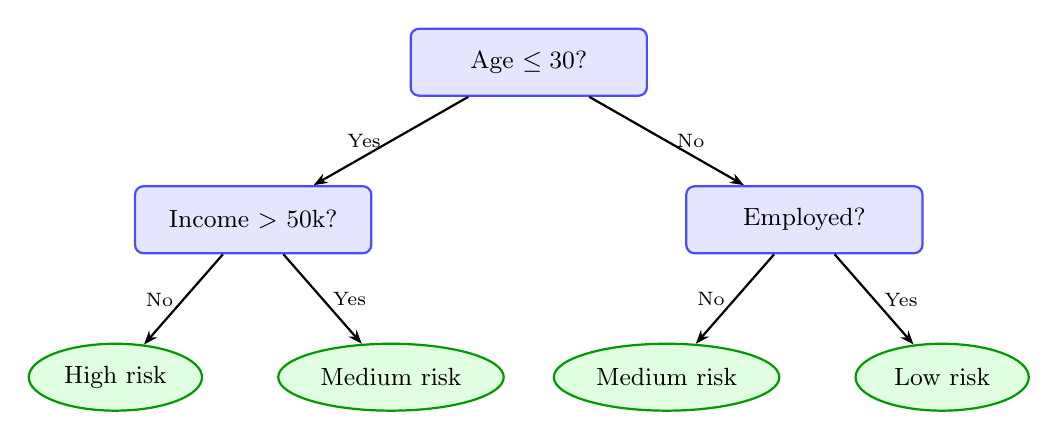
\begin{tikzpicture}[
  level 1/.style={sibling distance=7cm},
  level 2/.style={sibling distance=3.5cm},
  level distance=2cm,
]

  % Root
  \node[internal] (root) {Age $\leq 30$?}
    child[arrow] {
      node[internal] (young) {Income $>$ 50k?}
        child[arrow] {node[leaf] {High risk}  edge from parent node[edge label, left]{No}}
        child[arrow] {node[leaf] {Medium risk} edge from parent node[edge label, right]{Yes}}
      edge from parent node[edge label, left]{Yes}
    }
    child[arrow] {
      node[internal] (old) {Employed?}
        child[arrow] {node[leaf] {Medium risk} edge from parent node[edge label, left]{No}}
        child[arrow] {node[leaf] {Low risk}    edge from parent node[edge label, right]{Yes}}
      edge from parent node[edge label, right]{No}
    };

\end{tikzpicture}
\caption{Binary decision tree using TikZ \texttt{child} syntax.}
\end{figure}
\end{document}
